\documentclass{article}
\usepackage{amsmath}
\usepackage{graphicx}
\usepackage[colorlinks=true, linkcolor=blue, citecolor=black, backref=page]{hyperref}
\usepackage{lscape}
\usepackage{placeins}
\usepackage{booktabs}
\usepackage{listings}
\usepackage{xcolor}
\usepackage{float}
% Define custom colors
\definecolor{dkgreen}{rgb}{0,0.6,0}
\definecolor{gray}{rgb}{0.5,0.5,0.5}
\definecolor{mauve}{rgb}{0.58,0,0.82}

% Configure lstlisting settings for Python
\lstset{
  frame=tb,                      % Draw a frame at the top and bottom of the code block
  language=Python,               % Set the language to Python
  aboveskip=3mm,                 % Add space above the code block
  belowskip=3mm,                 % Add space below the code block
  showstringspaces=false,        % Do not display string spaces with special underlines
  columns=flexible,              % Allow flexible column spacing
  basicstyle={\small\ttfamily},  % Set the font style and size for code
  numbers=left,                  % Display line numbers on the left
  numberstyle=\tiny\color{gray}, % Style for line numbers
  keywordstyle=\color{blue},     % Style for keywords
  commentstyle=\color{dkgreen},  % Style for comments
  stringstyle=\color{mauve},     % Style for strings
  breaklines=true,               % Allow long lines to break
  breakatwhitespace=true,        % Break lines at whitespace if possible
  tabsize=4                      % Set tab size to 4 spaces
}

\begin{document}


\title{Task 4 -- NLO Lab Sheet 4}
\maketitle


\section{Best Fit Plot for Part 1(g)}

The nonlinear least squares model for radioactive decay is given by:  
\[
f(t; r_0, c_1, c_2, \lambda_1, \lambda_2) = r_0 + c_1 e^{-\lambda_1 t} + c_2 e^{-\lambda_2 t}
\]
with the following parameters:  
\[
r_0 = 3.5841, \quad c_1 = 2.8133, \quad c_2 = 2.8133, \quad \lambda_1 = 0.6959, \quad \lambda_2 = 0.6959
\]
indicating identical half-lives, leading to similar decay behavior. In the following plot we have the blue scatter points representing the observed radioactive level measurements over time and a red curve showing the best fit obtained using the above parameters.


\begin{figure}[H]
    \centering
    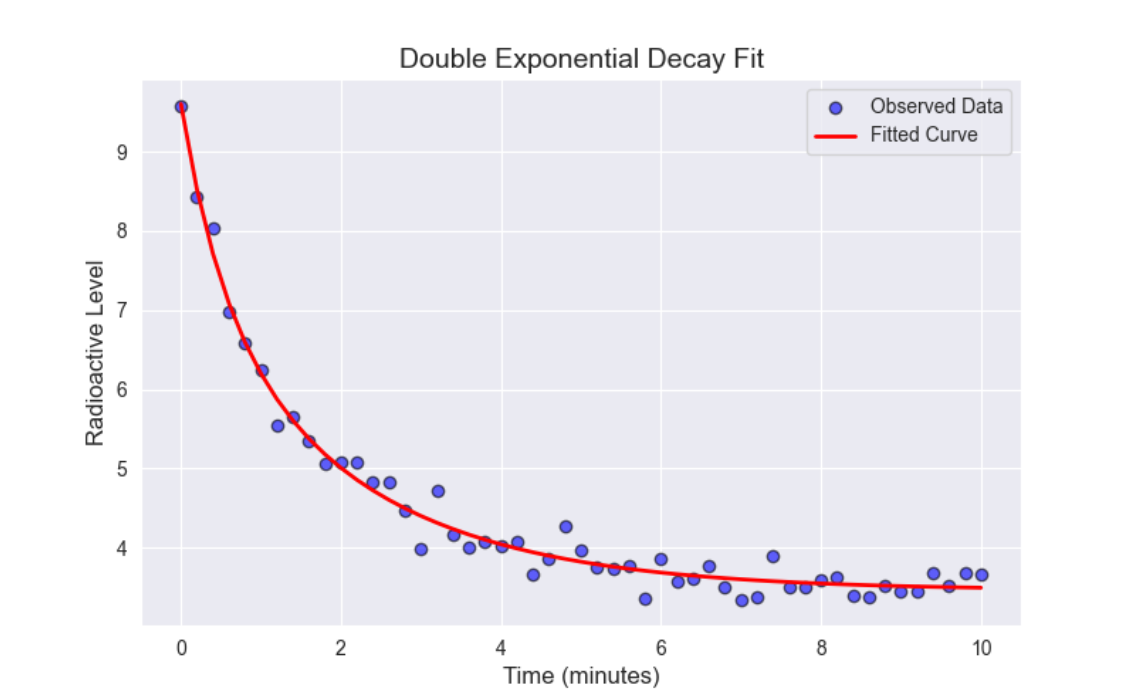
\includegraphics[width=1\textwidth]{NLO7.png}
\end{figure}


\section{Optimal Methods}

\subsection{Best Line Search Method}
The Quasi-Newton BFGS method with Armijo line search performs the best based on accuracy. However, the Gauss-Newton (GN) method with inertia correction also performs well resulting in a better overall solution. 

\subsection{Best Trust Region Method}
The Cauchy-Point or as called the Dog-leg (DL) method is significantly faster than the Levenberg-Marquardt (LM) method. The best combination is Dog-leg with Gauss-Newton, as it balances speed and accuracy. The DL with Newton method is even faster but can converge to a local minimum instead of the global one. 
\subsection{Conclusion}
It is possible for some methods to converge to a local minimum while others find the assumed global minimum. This property is not necessarily good neither is it bad given a particular method as it depends on the characteristic of the problem and initial conditions under which it operates and very arguably in most general sense one might be able to find required minima, may it be global or local. 
\newpage
\section{Computational Comparison}


\begin{table}[h]
    \centering
    \renewcommand{\arraystretch}{1.2}
    \begin{tabular}{lccc}
        \toprule
        \textbf{Method} & \textbf{Iterations} & \textbf{Function Evaluations} & \textbf{Final \( f \)} \\
        \midrule
        \multicolumn{4}{l}{\textbf{Trust Region (TR) Methods}} \\
        Newton + Cauchy-Point/Dog-Leg & 7 & 8 & 1.0946 \\
        Gauss-Newton + Cauchy-Point/Dog-Leg & 19 & 20 & 0.79835 \\
        Gauss-Newton + Levenberg-Marquardt & 29 & 29 & 0.79835 \\
        Newton + Levenberg-Marquardt & 25 & 26 & 0.79835 \\
        \midrule
        \multicolumn{4}{l}{\textbf{Line Search (LS) Methods}} \\
        BFGS (Armijo) & 14 & 43 & 1.0946 \\
        Gauss-Newton (Armijo) & 25 & 95 & 0.79835 \\
        Pollack-Riviere CG (Exact LS) & 27 & 790 & 1.0946 \\
        Fletcher-Reeves CG (Armijo) & 122 & 1090 & 1.0946 \\
        \bottomrule
    \end{tabular}
    \caption{Comparison of Trust Region and Line Search Methods}
    \label{tab:comparison}
\end{table}

\subsection{Analysis}

In terms if iterations efficiency (converging in a fewer iterations), the  Trust Region methods, particulary the Cauchy-Point(DL) performs  better. BFGS with Armijo LS balances speed and cost effectively. Dog-leg is fastest by iteration count, but BFGS is computationally more efficient. 



TR methods require Hessian evaluation, multiple linear system solutions per iteration, which is adds to computational expense. But line search methods, except for Newton, are more cost-efficient per iteration, depending just on the function and the gradient evaluation along with inexpensive direction determination.





\end{document}
